%%%%%%%%%%%%%%%%%%%%%%%%%%%%%%%%%%%%%%%%%%%%%%%%%%%%%%%%%%%%%%%%%%%%%
%% DRAFT -- Sequence asymmetry / interfacial potentials letter
%% Target: ACS Macro Letters (achemso class, journal=macl)
%% Built from idp_interface_manuscript_outline.md, idp_interface.md,
%% and the completed Step 1-3 results under results/ and figures/.
%% DDFT work is deliberately excluded per explicit instruction.
%%
%% Also TODO: the gamma ~ (Delta rho)^mu scaling claim (point 10 of the
%% outline) is stated qualitatively below since no exponent has been
%% fit yet against results/das_pappu_interfacial_tension.pdf's own data
%% -- fit mu before submission if this claim is to carry a number.
%%%%%%%%%%%%%%%%%%%%%%%%%%%%%%%%%%%%%%%%%%%%%%%%%%%%%%%%%%%%%%%%%%%%%
\documentclass[journal=macl,manuscript=article,layout=twocolumn]{achemso}
\SectionNumbersOff
\usepackage[version=3]{mhchem}
\usepackage{bm}

\author{Pierre J. Walker}
\email{pjwalker@caltech.edu}
\affiliation{Division of Chemistry and Chemical Engineering, California Institute of Technology, Pasadena, California, USA}

\title{Sequence Asymmetry Produces Interfacial Electrostatic Potentials in Polyampholytic Coacervates}

\abbreviations{IDP,LS,TPT,DFT,MSA}
\keywords{intrinsically disordered proteins, biomolecular condensates, liquid-state theory, classical density functional theory, interfacial electrostatics, sequence charge patterning}

\begin{document}

\begin{abstract}
Biomolecular condensates formed by intrinsically disordered proteins (IDPs) are increasingly implicated in setting up electrostatic potentials at their interface with the surrounding cytoplasm, with consequences ranging from cellular electrochemical signaling to interfacial catalysis. Using a classical density functional theory (DFT) extension of liquid-state (LS) theory, we compute the interfacial structure of net-neutral, equal-charge polyampholyte sequences along their full liquid-liquid coexistence boundary and show that whether an interface carries a potential at all is controlled not by the conventional charge-patterning parameter $\kappa$, but by a distinct, exactly defined symmetry property of the sequence. Reversing a linear chain's bead order is always a symmetry of its neutral packing and connectivity; for an \emph{anti-palindromic} sequence -- any clean diblock or strictly alternating pattern -- that same relabeling is also exactly a global charge inversion, which forces the interfacial charge density, and hence the electrostatic potential, to vanish identically regardless of $\kappa$. We introduce a windowed order parameter $\xi$ that measures local departure from this anti-palindrome condition, and show across a survey of sequences at fixed coupling strength that $\xi$ organizes the achievable interfacial potential far more cleanly than $\kappa$ does. Finally, we show that introducing a symmetric pair of mobile ions preserves a nonzero interfacial potential -- as it must, given charge neutrality of each bulk phase -- but converts the salt-free step into a double-layer-like profile whose decay length tracks the screening length of each adjoining phase. These results identify the minimal sequence requirement for a net-neutral polyampholyte to generate its own interfacial electrostatic potential.
\end{abstract}

\maketitle
% The introduction needs a more polymer-physics-oriented opening, perhaps even focusing on electrostatic potentials at interfaces in general, and then zooming in on polyelectrolytes more broadly and then specific applications like biological applications.
Many eukaryotic cells organize their biochemistry not only through membrane-bound organelles but also through membraneless compartments that assemble via liquid-liquid phase separation \cite{hymanLiquidLiquidPhaseSeparation2014,bananiBiomolecularCondensatesOrganizers2017}. These biomolecular condensates, exemplified by the nucleolus and other ribonucleoprotein granules \cite{brangwynneActiveLiquidlikeBehavior2011,nottPhaseTransitionDisordered2015}, concentrate specific proteins and nucleic acids to compartmentalize cellular biochemistry, and their assembly and dissolution respond sensitively to the surrounding chemical environment, including pH, temperature, pressure, and ionic strength \cite{cinarPressureInducedDissolutionReentrant2018,albertiCurrentPracticesStudy2025}. Intrinsically disordered proteins (IDPs), which lack a stable folded structure and instead behave as flexible polyampholyte-like chains, are frequent drivers of this behavior \cite{uverskyIntrinsicallyDisorderedProteins2015}.

Interfacial electrostatic potentials formed by coacervates of polyelectrolytes and IDPs are of growing interest for understanding how these condensates and related membraneless assemblies interact with their environment \cite{daiBiomolecularCondensatesRegulate2024,daiUnlockingElectrochemicalFunctions2024}. Beyond cellular electrochemistry, such interfacial potentials have attracted attention for applications including the use of condensate and droplet interfaces as catalytic environments \cite{chenBiomolecularCondensatesCan2026}. The electrostatic structure of interfaces is comparatively well understood for simple electrolyte mixtures and for less trivial cases such as neutral polar fluids and water \cite{varnerStockmayerFluidShifted2026,walkerStockmayerFluidShifted2026a}, but biomolecular condensates are substantially more complex: their constituent macromolecules carry intricate, sequence-dependent charge patterns, and the resulting interfaces depend sensitively on external factors such as pH, temperature, and salt concentration.

The distribution of charged residues along an IDP's sequence, not merely its net charge or composition, is a key determinant of both single-chain conformations and phase behavior \cite{dasConformationsIntrinsicallyDisordered2013,dasRelatingSequenceEncoded2015,sawleTheoreticalMethodCompute2015}. The charge-patterning parameter $\kappa$ introduced by Das and Pappu \cite{dasConformationsIntrinsicallyDisordered2013} and the related sequence-charge-decoration measure of Sawle and Ghosh \cite{sawleTheoreticalMethodCompute2015} quantify how segregated oppositely charged residues are along a chain, and both correlate strongly with a polyampholyte's propensity to self-coacervate \cite{linSequenceSpecificPolyampholytePhase2016,pakSequenceDeterminantsIntracellular2016}: more blocky sequences phase-separate more readily and with sharper interfaces, a trend reproduced across theory, simulation, and experiment and reviewed extensively elsewhere \cite{linTheoriesSequenceDependentPhase2018,holehouseCIDERResourcesAnalyze2017,ghoshRulesPhysicalMathematics2022}. Yet $\kappa$ was derived to organize single-chain dimensions and the bulk phase boundary, not interfacial structure, and whether it -- or any related descriptor -- also controls finer electrostatic features of the interface itself has not been established.

Because of this complexity, it is useful to develop reduced representations. A common one treats an IDP as a polyelectrolyte chain of identically sized, oppositely charged beads, reducing its identity to a composition and a charge-patterning sequence \cite{dignonSequenceDeterminantsProtein2018}. Molecular dynamics simulations provide the most complete description of such a system but remain computationally limited in resolving interfaces, let alone any interfacial potential it carries, for macromolecules of realistic length\cite{anEffectsChargeAsymmetry2024,zhouSequenceLengthscaleDependent2026,wangSequencedependentConformationalTransitions2024,leeRoleChargeSequence2024,dignonTemperatureControlledLiquidLiquid2019}. Analytical theory offers a practical alternative, and a range of complementary frameworks has been developed for polyelectrolyte and polyampholyte coacervation, including field-theoretic simulation \cite{leeComplexCoacervationField2008,mccartyCompletePhaseDiagram2019,danielsenSmallIonEffects2019,danielsenMolecularDesignSelfcoacervation2019}, the polymer reference interaction site model \cite{perryPRISMBasedTheoryComplex2015}, and the random phase approximation \cite{borueStatisticalTheoryGlobular1990,castelnovoComplexationOppositelyCharged2001,danielsenMolecularDesignSelfcoacervation2019,rumyantsevUnifyingWeakStrong2022}, surveyed recently by Rumyantsev \textit{et al.} \cite{rumyantsevPolyelectrolyteComplexCoacervates2021}. Among these, self-consistent field theory's well-known limitations in reproducing the phase behavior of coarse-grained polyampholytes make it ill-suited here, whereas liquid-state (LS) theory -- specifically the variant of Zhang \textit{et al.}, built on the mean-spherical approximation (MSA) -- has had considerable success reproducing both the phase and interfacial behavior of such systems \cite{zhangSaltingOutSaltingInPolyelectrolyte2016,wangInterfacialTensionsPolyelectrolyte2024,leeRoleChargeSequence2024}.

We extend this LS theory to a classical density functional theory\cite{jiangMicroscopicInsightsElectrochemical2013,jiangDensityFunctionalTheory2011,gallegosHierarchicalModelWeak2023,gallegosThermodynamicNonidealityCharge2021,gallegosIsingDensityFunctional2021,jiangDensityFunctionalTheory2018} (DFT) capable of resolving the full, sequence-specific spatial structure of a planar liquid-liquid interface, rather than treating the chain only at the level of a bulk equation of state. The reduced free energy is decomposed into four contributions,
\begin{equation}
    f = \frac{F}{Vk_\mathrm{B}T} = f_\mathrm{id.} + f_\mathrm{hs} + f_\mathrm{chain} + f_\mathrm{el.}\,,
    \label{eq:four-terms}
\end{equation}
% In this section here, details need to be provided as to how each term was extended to classical DFT. E.g. FMT was used for the hard-sphere term, and MSA was used for the electrostatic term. The ideal term is already a functional of the density profile, so it does not require any extension.
% We also need to provide details regarding how connectivity was enforced (i.e. using a propagator) and the settings used for converging these calculations. Add a reference to SI for the full set of equations.
an ideal (translational) term, a Boublík--Mansoori--Carnahan--Starling--Leland hard-sphere term for excluded volume, a first-order thermodynamic perturbation theory (TPT1) term for tangent-bead chain connectivity \cite{wertheimFluidsHighlyDirectional1984,wertheimFluidsHighlyDirectional1984a,wertheimFluidsHighlyDirectional1986,wertheimFluidsHighlyDirectional1986a}, and an MSA term \cite{blumMeanSphericalModel1975} for electrostatic correlations under a constant-dielectric (primitive-model) solvent. All beads -- charged and neutral, chain and small-ion -- share a common diameter $\sigma=3\times10^{-10}\,\mathrm{m}$. Spatial density profiles $\rho_k(\mathbf{r})$ for each bead type $k$ are obtained self-consistently from the Euler-Lagrange fixed-point equation,
\begin{multline}
    \rho_k(\mathbf{r}) = \rho_k^\mathrm{b}\exp\!\Bigg[-\beta\Bigg(\frac{\delta F_\mathrm{res}[\rho]}{\delta\rho_k(\mathbf{r})} \\
    - \frac{\delta F_\mathrm{res}[\rho]}{\delta\rho_k(\mathbf{r})}\bigg\vert_{\rho^\mathrm{b}} - Z_k e\,\psi(\mathbf{r})\Bigg)\Bigg]\,,
    \label{eq:fixedpoint}
\end{multline}
where $\rho_k^\mathrm{b}$ is the bulk density of species $k$ in the phase used as the profile's reference, $Z_k$ is its valence, and $\psi(\mathbf{r})$ is the self-consistent electrostatic potential. The bulk equation of state, Eq.~\ref{eq:four-terms}, and the spatial functional, Eq.~\ref{eq:fixedpoint}, were cross-validated against one another to machine precision before use.

We first consider the five canonical 50-bead sequences sv10, sv15, sv20, sv25, and sv30 from Das and Pappu\cite{dasConformationsIntrinsicallyDisordered2013}, each net-neutral with 25 positive and 25 negative beads, spanning the sequence-disorder parameter $\kappa$ (the Das--Pappu/Sawle--Ghosh local charge-clustering order parameter \cite{dasConformationsIntrinsicallyDisordered2013,sawleTheoreticalMethodCompute2015}) from $0.163$ (sv10) to $1.0$ (sv30, the perfect diblock). These five were chosen as standard benchmarks for sequence-patterning and because they span essentially the full accessible range of $\kappa$ at fixed composition and chain length, letting us isolate the effect of patterning from that of net charge or chain length.

\begin{figure*}[t]
    \centering
    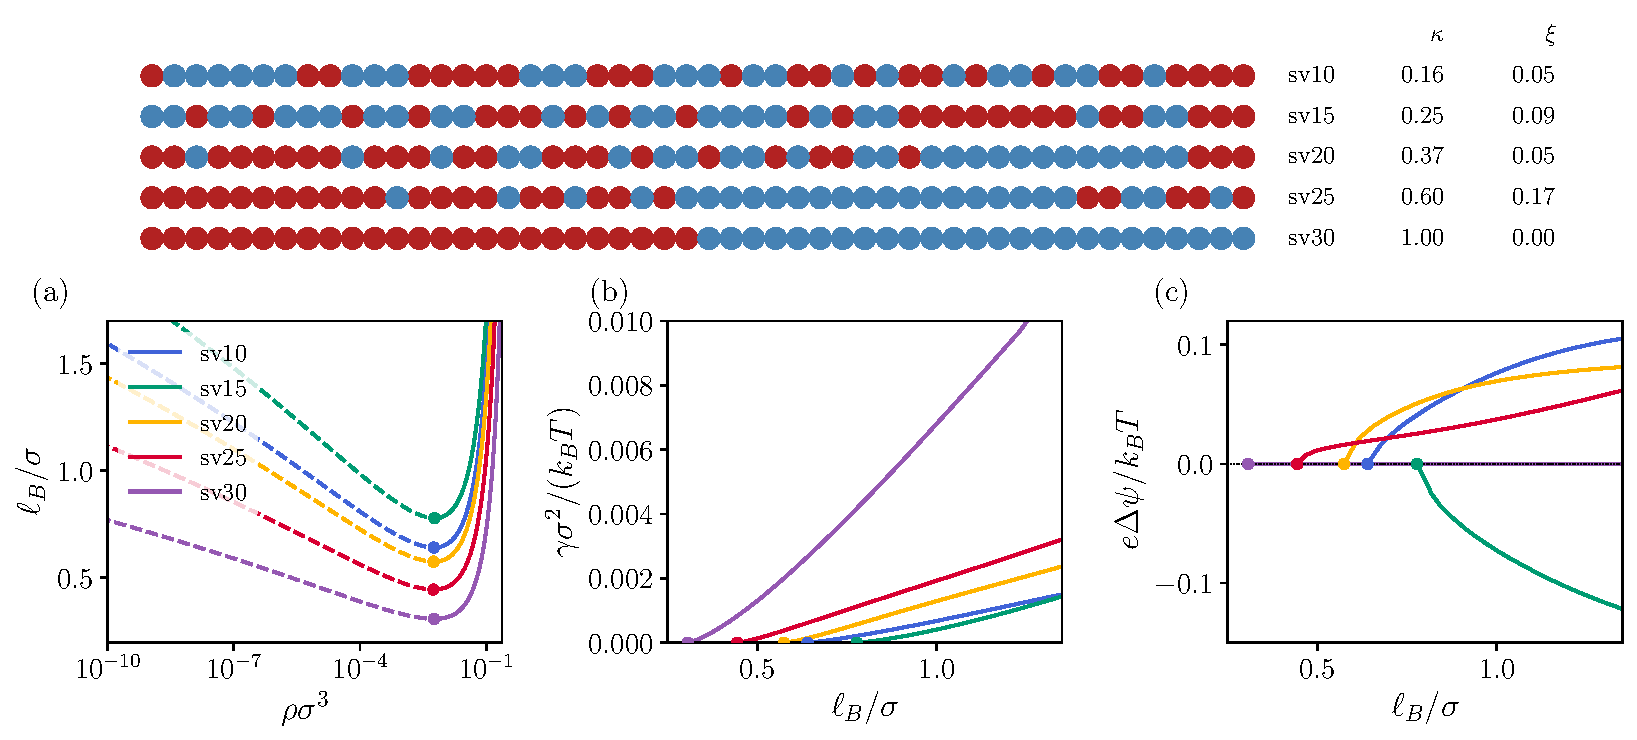
\includegraphics[width=\linewidth]{figures/manuscript_fig1.pdf}
    \caption{Sequence patterning strip and (a) bulk phase diagram, (b) interfacial tension $\gamma$, and (c) the electrostatic potential difference $e\Delta\psi/k_\mathrm{B}T$ ($\Delta\psi\equiv\psi_\mathrm{sup}-\psi_\mathrm{dense}$, supernatant minus dense), all traced along each sequence's own two-phase coexistence boundary, for the five sv10/15/20/25/30 sequences.}
    \label{fig:1}
\end{figure*}

Tracing each sequence's own two-phase coexistence boundary, we find the expected qualitative trend in Figure~\ref{fig:1}a: more ordered sequences phase-separate more readily, lowering the critical Bjerrum length $\ell_{\mathrm{B},c}$. This is expected as sequences with more segregated charges should experience stronger electrostatic interactions and thus phase-separate more readily. This monotonic trend in $\kappa$, however, is not perfect: sv10 ($\kappa=0.16$, $\ell_{\mathrm{B},c}/\sigma=0.640$) and sv15 ($\kappa=0.25$, $\ell_{\mathrm{B},c}/\sigma=0.778$) seemingly break this trend. While it is known that $\kappa$ is an imperfect predictor of phase behavior, this reflects a limitation in the TPT1 chain treatment's of only accounting for nearest-neighbor bonded correlations.

This same ordering is reflected directly in the interfacial tension (Figure~\ref{fig:1}b), consistent with the expected scaling $\gamma\propto(\Delta\rho)^\mu$ relating tension to the density difference $\Delta\rho$ between the coexisting phases\cite{macleodRelationSurfaceTension1923,guggenheimPrincipleCorrespondingStates1945,rowlinsonMolecularTheoryCapillarity2002}: the most ordered sequence (sv30) separates the most sharply and carries the largest tension at a given $\ell_\mathrm{B}$, while sv10 and sv15, the two lowest-$\kappa$ sequences, trace nearly indistinguishable, shallow curves.

\begin{figure*}[t]
    \centering
    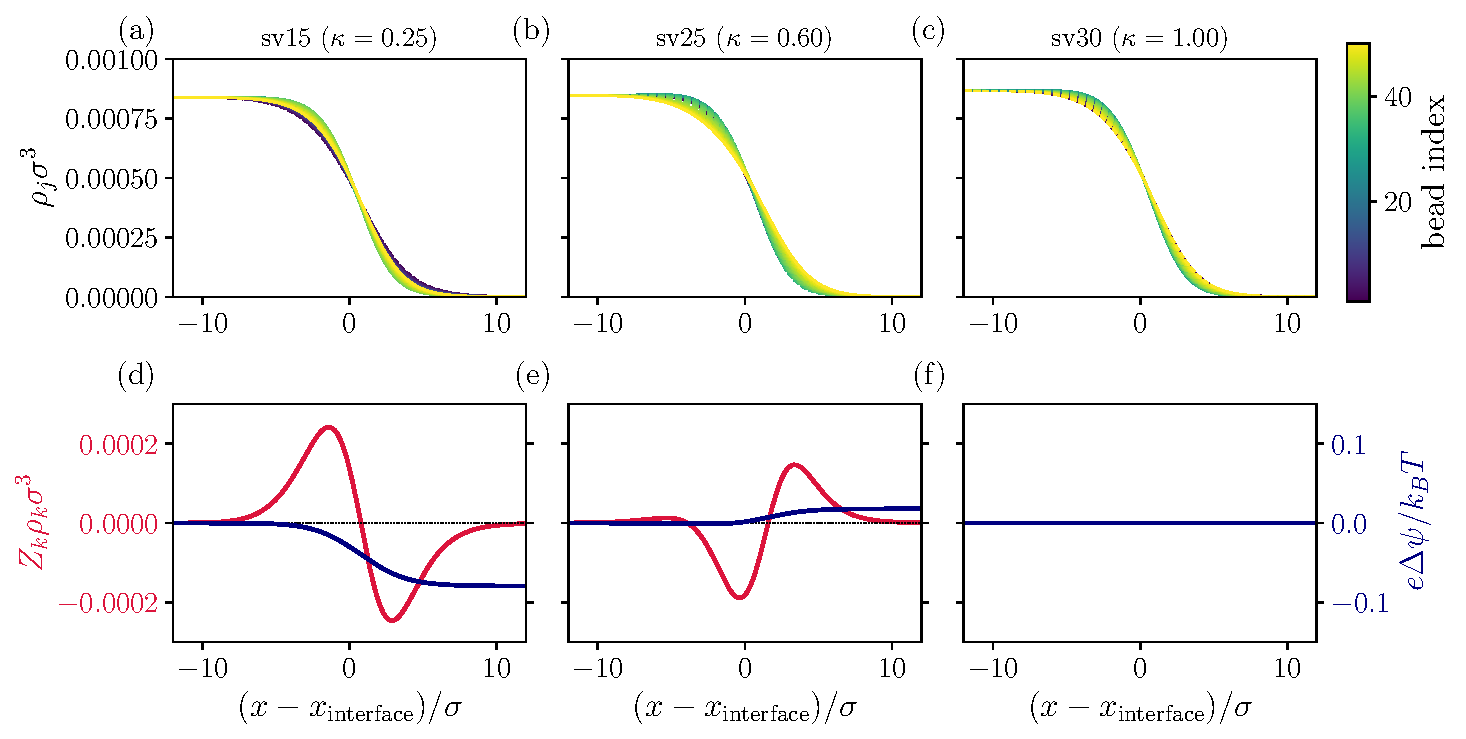
\includegraphics[width=\linewidth]{figures/manuscript_fig2.pdf}
    \caption{For sv15, sv25, and sv30 (the three sequences discussed in the main text), respectively: (a-c) bead-resolved density profiles across the interface at $\ell_\mathrm{B}/\sigma=1$, colored by bead index (solid: $Z=+1$, dashed: $Z=-1$); (d-f) net charge density (left axis) and electrostatic potential difference $e\Delta\psi/k_\mathrm{B}T$ (right axis) over the same window.}
    \label{fig:2}
\end{figure*}

These bulk-level trends are mirrored at the level of individual beads (Figure~\ref{fig:2}a-c): interfaces sharpen with increasing $\kappa$, as expected. Another observation is that sv30, the perfect diblock, shows no distinction whatsoever between its cationic and anionic halves as the two sub-profiles overlap exactly. This is due to the symmetry in the chemical environments between bead $i$ and the oppositely charged bead $N-i+1$. This symmetry results in perfect cancelling of charge and, thus, no electrostatic potential (Figure~\ref{fig:2}f). On the other hand, this symmetry in local environments is broken within sv15 and sv25, resulting in both developing nonzero charge density profiles and correspondingly nonzero electrostatic potentials. Interestingly, while sv25 does have the sharper interface and the larger interfacial tension, its resulting electrostatic potential potential is lower in magnitude than sv15. This is the first indication that the strength of this electrostatic potential may not correlate directly with the sequence disorder metric, $\kappa$.
% I think these last sentences need clarification as it is not clear why one would expect a greater electrostatic potential from a sharper interface. My logic is that with a faster decrease in density profiles, if there is a net charge profile, then its profile should also be sharper and greater. This is not the case. One case also point to the existence of three large extrema in sv25 compare to sv15's two.

Even more perculiar is that, while both sequences are neutral, the sign of the electrostatic potential profile is opposite. This distinction can be rationalized directly from differences in local chain environment: between sv15 and sv25, the \emph{sign} of the resulting potential corresponds closely to the sign of the largest locally ordered region. Examining Figure~\ref{fig:1}, one can see that for sv15, its largest ordered block is cationic whilst for sv25, it is anionic. These blocks will preferentially adsorb towards the coacervate phase, leaving the oppositely-charged regions to adsorb preferentially towards the supernatant, as reflected in Figures~\ref{fig:2}(d) and Figures~\ref{fig:2}(e). 

since the weaker cohesive attraction of a disordered domain favors its preferential adsorption at the interface. Figure~\ref{fig:1}c shows this concretely: sv30 never generates a potential at any $\ell_\mathrm{B}$, while all four other sequences do. The strength of that potential, however, is not monotonic in $\kappa$ at all (if anything, it is weakly \emph{anti}-correlated with it over this family) -- sv15 carries the largest-magnitude potential found anywhere in this set, and sv25, despite its substantially higher $\kappa$, one of the smallest. Some aspect of sequence patterning not captured by $\kappa$ alone is clearly responsible.

We identify that aspect as a symmetry property of the sequence. Reversing a linear chain's bead order, $i\leftrightarrow N+1-i$, is always a symmetry of the neutral hard-sphere and chain-connectivity physics in Eq.~\ref{eq:four-terms} -- a tangent-bead chain has no intrinsic direction. For an \emph{anti-palindromic} sequence, $Z_i=-Z_{N+1-i}$ for every bead (true of any clean diblock, and of strict alternation), that same relabeling is \emph{also} exactly a global charge inversion. Combined, the two symmetries force the net local charge density to equal its own negative at every point in space -- i.e., to vanish identically -- independent of how strongly segregated the sequence is. A \emph{true palindrome}, $Z_i=+Z_{N+1-i}$, inherits the same relabeling symmetry but not the accompanying charge flip, so nothing forces a cancellation; such a sequence can carry a substantial potential despite often modest $\kappa$.

We encode this with a windowed order parameter,
\begin{equation}
    \xi = \frac{1}{\xi_\mathrm{max}(N)}\sum_{j=1}^{N-w+1}\left(\sum_{i=j}^{j+w-1}\big(Z_i+Z_{N+1-i}\big)\right)^{\!2}\,,
    \label{eq:xi}
\end{equation}
with window size $w=6$ beads, normalized by $\xi_\mathrm{max}(N)$, the true combinatorial maximum achievable for a sequence of that length and net charge (not a loose analytic bound), so that $\xi\in[0,1]$ with $1$ genuinely reachable. Each inner summand $Z_i+Z_{N+1-i}$ vanishes exactly whenever bead $i$ and its mirror partner $N+1-i$ are anti-paired -- the specific condition protecting the zero-potential result above -- so $\xi$ measures local departure from the anti-palindrome condition along the chain, rather than global charge clustering.

\begin{figure}[ht!]
    \centering
    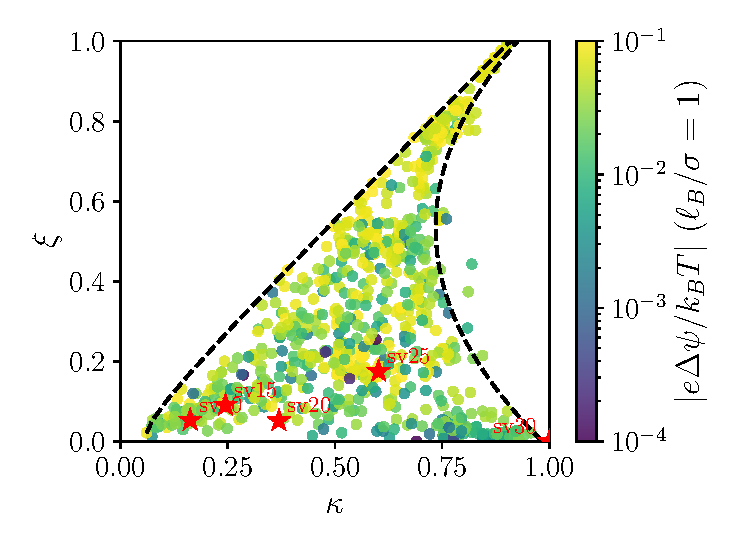
\includegraphics[width=\linewidth]{figures/neutral_sample_50mer_scatter_kappa_kappasym.pdf}
    \caption{$\kappa$ vs. $\xi$ for a broad survey of net-neutral 50-bead sequences at fixed $\ell_\mathrm{B}/\sigma=1$, colored by $|\Delta\psi|$, the magnitude of the resulting interfacial potential step (symlog scale); the five sv10/15/20/25/30 sequences are marked. The dashed envelope is the combinatorially achievable upper bound on $\xi$ at each $\kappa$, derived independently of this sampled data.}
    \label{fig:3}
\end{figure}

Having established the exact symmetry condition responsible for a zero potential, we next ask how it organizes a much broader survey of sequences. Figure~\ref{fig:3} samples many more sequences at fixed coupling ($\ell_\mathrm{B}/\sigma=1$) and plots them in the $(\kappa,\xi)$ plane. At $\xi=0$, the interfacial potential is always exactly zero, for every value of $\kappa$ -- the charges in the polyampholyte cancel perfectly at the interface regardless of how blocky the sequence otherwise is. At high $\kappa$, $\xi$ becomes a strong, almost sufficient determinant of the resulting potential strength. We note, too, that $\kappa$ and $\xi$ are not fully orthogonal descriptors: the envelope visible in Figure~\ref{fig:3} bounds the region of $(\kappa,\xi)$ space that is combinatorially achievable at all, so the two parameters cannot be explored fully independently of one another.

Interestingly, at lower $\kappa$ and higher $\xi$, the achievable potential strength appears to increase further still, plausibly because the wider interfaces found at lower $\kappa$ allow a more spatially extended, and therefore more consequential, nonzero charge profile to develop at the interface. This echoes the markedly non-trivial relationship we previously found between charge asymmetry and interfacial potential strength in asymmetric dipolar fluids \cite{varnerStockmayerFluidShifted2026,walkerStockmayerFluidShifted2026a}. Nonetheless, like $\kappa$, $\xi$ remains an imperfect predictor and does not by itself fully collapse the data in Fig.~\ref{fig:3} -- a limitation that may again trace back to the TPT1 chain treatment, which could in principle be extended to include higher-order (e.g., triplet) intrachain correlations.

\begin{figure*}[t]
    \centering
    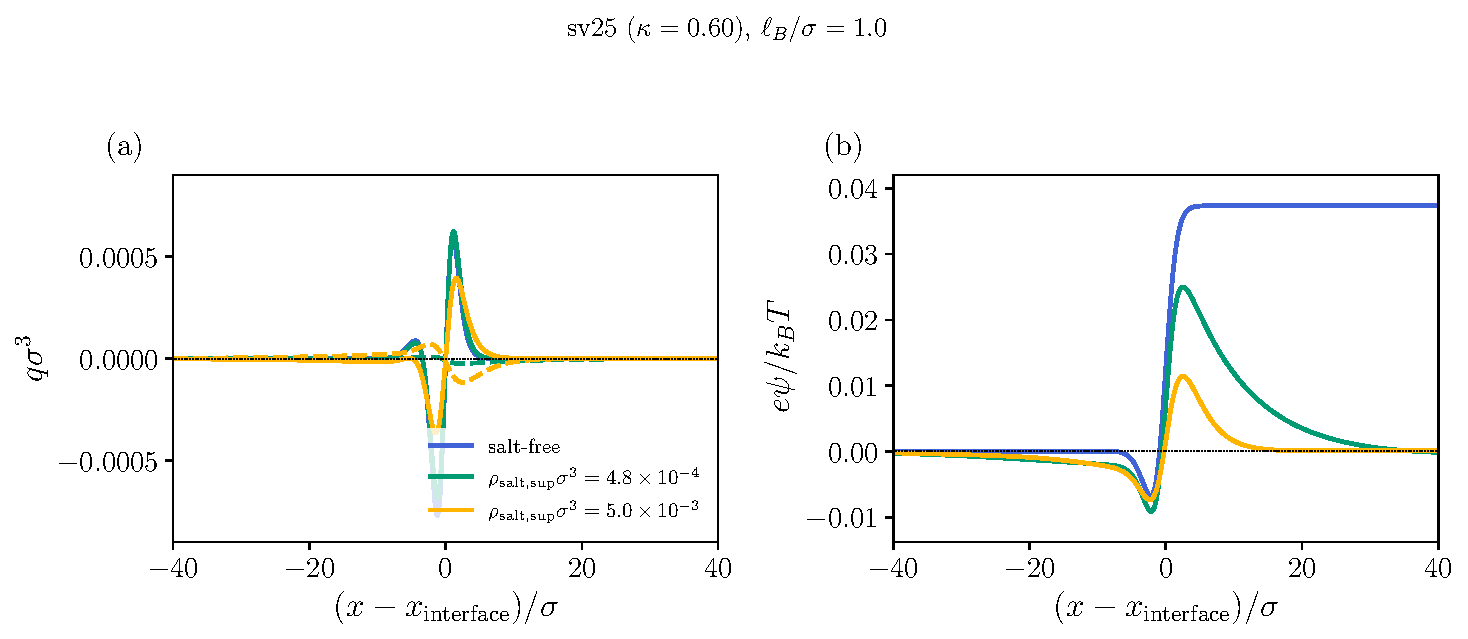
\includegraphics[width=\linewidth]{figures/manuscript_fig4.pdf}
    \caption{For sv25 at $\ell_\mathrm{B}/\sigma=1$, salt-free and with a symmetric monovalent salt added at two reduced salt densities in the supernatant, $\rho_{\mathrm{salt,sup}}\sigma^3$: (a) net charge density of the chain (solid) and of the combined mobile ions (dashed; salt-free has none), on the same axis -- the ion response is visibly far smaller than the chain's own charge imbalance; (b) electrostatic potential profile. The interfacial potential step persists with added salt but decays into each bulk phase over a finite length, markedly longer on the supernatant side.}
    \label{fig:4}
\end{figure*}

Having established the minimal sequence requirement for a salt-free interfacial potential, we next ask what happens when a symmetric pair of mobile ions is introduced -- a question our earlier dipolar-fluid work \cite{varnerStockmayerFluidShifted2026,walkerStockmayerFluidShifted2026a} did not address. By construction, once such a system phase-separates, the electrostatic potential difference between the two bulk phases must remain exactly zero, or charge neutrality in each phase would be violated. Figure~\ref{fig:4} shows that the interfacial potential nonetheless survives: rather than stepping directly between two flat, zero-difference plateaus, it now decays slowly into each bulk phase, reminiscent of a classical electrical double layer \cite{gouyConstitutionChargeElectrique1910,debyeZurTheorieElektrolyte1923}. This decay is set by the screening length within each phase, and is correspondingly much slower in the supernatant, where the screening ion density -- and hence the local Debye length's inverse -- is far smaller than in the dense, polyampholyte-rich coacervate phase.

\begin{figure}[ht!]
    \centering
    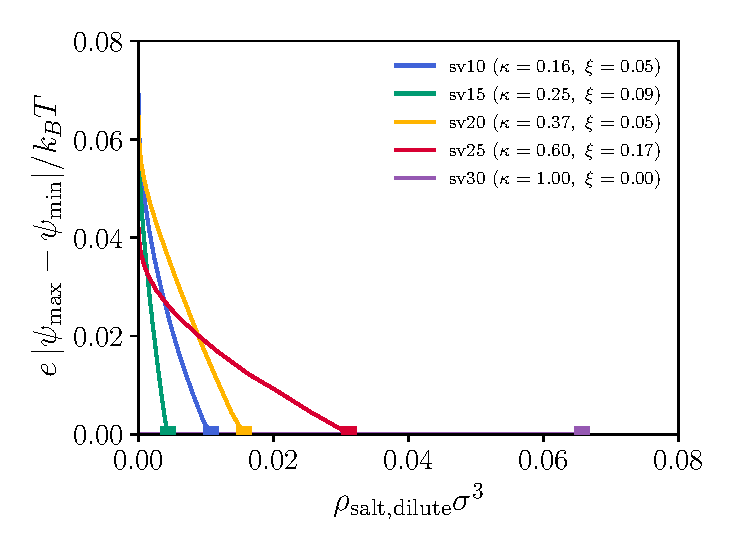
\includegraphics[width=\linewidth]{figures/das_pappu_saltsweep_dpsi_vs_rhosalt.pdf}
    \caption{Electrostatic potential step $e|\Delta\psi|/k_\mathrm{B}T$ against the dilute-phase (supernatant) salt density $\rho_{\mathrm{salt,dilute}}\sigma^3$ for all five sv10/15/20/25/30 sequences at $\ell_\mathrm{B}/\sigma=1$, each traced from the salt-free limit to its own exact critical point (square marker), where the two phases -- and hence $\Delta\psi$ -- merge identically to zero. sv30's curve is identically zero at every salt concentration, not only salt-free, consistent with its exact anti-palindrome symmetry.}
    \label{fig:5}
\end{figure}

The same salt-screening effect, traced now along the full liquid-liquid coexistence boundary rather than at a single, fixed composition, is summarized in Figure~\ref{fig:5} for all five sequences. For sv10, sv15, sv20, and sv25, $|\Delta\psi|$ falls monotonically from its salt-free value and reaches exactly zero as the dilute-phase salt density approaches each sequence's own critical value $\rho_{\mathrm{salt},c}$, where the dense and dilute phases become indistinguishable and no interface -- and so no interfacial potential -- remains. sv30 requires no such approach to criticality to reach zero: its exact anti-palindrome symmetry forces $\Delta\psi\equiv0$ at every salt concentration sampled, salt-free included, exactly as Figure~\ref{fig:2}f already showed at a single composition. The ordering of the four nonzero curves away from criticality follows the same $\xi$-controlled trend established in Figure~\ref{fig:3} rather than $\kappa$: sv25, the highest-$\xi$ sequence of the family ($\xi=0.17$), sustains a nonzero potential out to by far the highest salt density of the four ($\rho_{\mathrm{salt},c}\sigma^3=0.031$, roughly double sv20's $0.016$ and triple sv10's $0.011$), despite starting from the lowest salt-free potential of the four ($e\Delta\psi/k_\mathrm{B}T=0.044$ at $\rho_{\mathrm{salt,dilute}}=0$, versus $0.077$ for sv10 and $0.070$ for sv20).

Together, these results identify the minimal sequence requirement for a net-neutral polyampholyte to generate an electrostatic potential at its own interface: a nonzero $\xi$, i.e., a real, local departure from the anti-palindrome condition that otherwise forces exact cancellation regardless of sequence blockiness or salt concentration. Several extensions follow naturally from this minimal picture, including the effect of additional non-idealities such as short-range ($\chi$-type) and hydrogen-bonding interactions, and the consequences for condensate formation dynamics: even when a growing condensate's bulk composition remains net-neutral, a nonzero interfacial charge may introduce an electrostatic barrier that resists the coalescence and coarsening of smaller droplets into larger ones.

\begin{acknowledgement}
TODO (Pierre): funding sources, computational resources, and any additional acknowledgments.
\end{acknowledgement}

\bibliography{literature/references/references}

\end{document}
